%!TEX root = ../report.tex

\chapter{DCNN and Semantic Segmentation}

	In this chapter, we look into the basic concepts of neural networks and later, how such concepts have been used for the task of semantic segmentation. In section  \textbf{[todo]}

\section{Artificial Neural Networks}

Artificial Neural Networks (ANN), inspired by the neural networks in our brain, was designed to learn tasks without explicitly programming descriptive features of the concerned tasks. An ANN is made up of processing units called neurons which performs a non-linear transformation, using an activation function, of the weighted linear combination of inputs. Figure \ref{Fig:haykin_ann_n} illustrates a non-linear model of a neuron. Many such neurons are connected to one another in an ANN resulting in its ability to learn highly non-linear function mappings from input to output space. Figure \ref{Fig:haykin_ann_ml} illustrates a multilayer feedforward neural network.

	\begin{figure}
		\centering
		\begin{subfigure}{.5\textwidth}
			\centering
			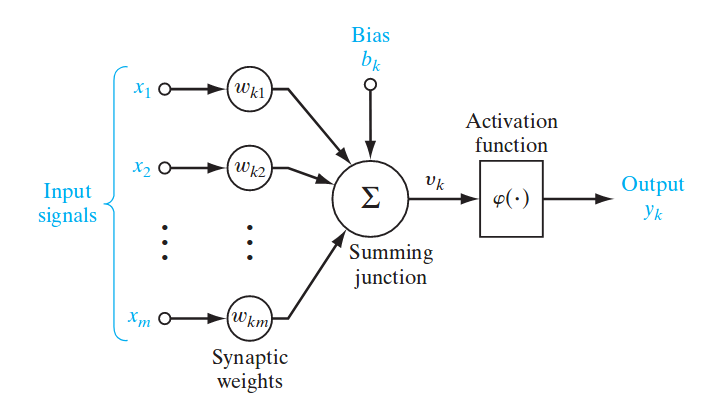
\includegraphics[width=1\linewidth]{images/neuron}
			\caption{}
			\label{Fig:haykin_ann_n}
		\end{subfigure}
		\begin{subfigure}{.3\textwidth}
			\centering
			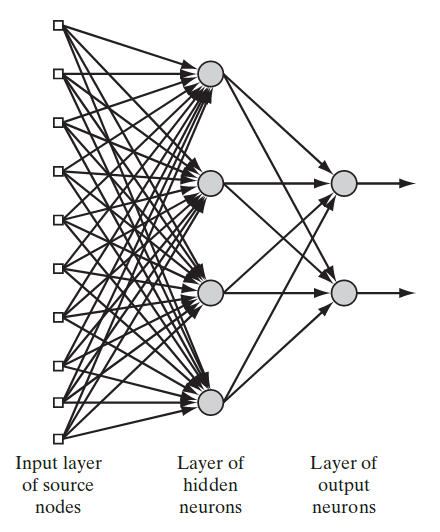
\includegraphics[width=1\linewidth]{images/ml_ff_nn}
			\caption{}
			\label{Fig:haykin_ann_ml}
		\end{subfigure}
		\caption{(a) A non-linear neuron model. $v_k$ = $\sum_{i=1}^{m} w_{ki} x_i$ denotes the local field of the neuron, $\varphi$ is the activation function and $y = \varphi(v_k)$ is the output of the neuron. (b) An illustration of a multilayer feedforward neural network with input source nodes, one hidden layer of neurons and an output layer of neurons \cite{haykin}.}
		\label{Fig:haykin_ann}
	\end{figure}
	
\subsection{Universal approximation theorem}


%\subsection{Multilayer Perceptron}

%The Multilayer Perceptron (MLP) is a feedforward neural network with at least one layer in addition to an input and an output layer. The additional layers lie in between the input and the output layers and are called hidden layers. The input layer 

\section{Convolutional Neural Networks}

Convolutional Neural Networks (CNNs or Conv Nets) are a class of feedforward neural networks which are used in the field of computer vision. Tasks such as image classification, object detection and semantic segmentation make use of CNNs. Unlike the multilayer feedforward network shown in Figure \ref{Fig:haykin_ann_ml}, CNNs are designed to handle image data which is usually represented as a stack of 2 dimensional values. A major part of CNNs comprise the use of convolutional layers which greatly reduce the number of parameters in comparison to fully-connected layers.

\subsection{Covolution theorem}

\subsection{CNN Architecture}

An RGB image typically consists of height, width and 3 channels representing red, blue and green. In order to better handle this structure of an input image, the neurons in a convolutional layer are arranged in a 3D volume of height, width and depth. An illustration of the 3D arrangement of neurons can be seen in Figure \ref{Fig:cnn_neuron}. The general architecture of a CNN is illustrated in Figure \ref{Fig:cnn_arch}. A CNN is composed of different layer types such as convolutional layer, pooling layer, normalization layer and pooling layer. Each of the layers are looked into in detail in the subsequent sections.

	\begin{figure}[h]
		\centering
		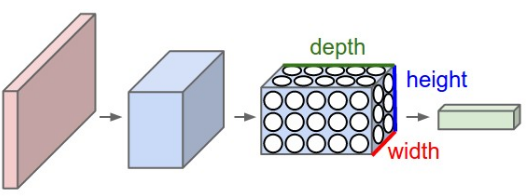
\includegraphics[width=.4\linewidth]{images/conv_3dneurons}
		\caption{Illustration of 3D (height, width, depth) arrangement of neurons in a convolutional layer. The convolutional layer transforms a 3D input volume to a 3D output volume  \cite{cs231n}.}
		\label{Fig:cnn_neuron}
	\end{figure}
	
	\begin{figure}[h]
		\centering
		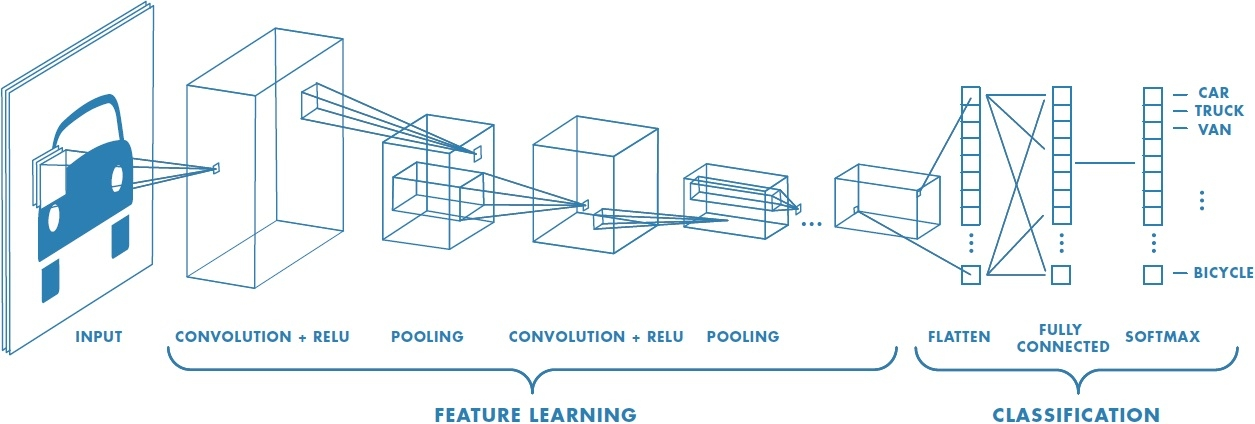
\includegraphics[width=1\linewidth]{images/cnn_matlab}
		\caption{This figure illustrates a CNN architecture. A convolution layer convolves on the input image or feature maps followed by an ReLU activation which produces output feature maps. A pooling layer downsamples feature maps. The CNN architecture performs feature learning and classification \cite{matlab_cnn}.}
		\label{Fig:cnn_arch}
	\end{figure}

\subsubsection{Convolutional layer}



\subsubsection{Pooling layer}

\subsubsection{Normalization layer}

\subsubsection{Fully-connected layer}

\section{Deep Learning for Semantic Segmentation}

